\documentclass[journal,12pt,twocolumn]{IEEEtran}

\usepackage{graphicx}
\graphicspath{ {./5609/Assign3/} }

\usepackage{amsmath}
\newcommand{\myvec}[1]{\ensuremath{\begin{pmatrix}#1\end{pmatrix}}}
\title{Assignment 3}
\author{PARIMISETTY HARINADHA (CS19RESCH11004)}
\begin{document}
\maketitle
\newpage
\begin{abstract}
This document calculate the circle equation such that circle is passing through given two points and the centre of the circle is placed on given straight line.
\end{abstract}
Download all python codes from 
\framebox[1\width]{ https://github.com/cs19resch11004/hari }
Download all Latex-tikz codes from 
\framebox[1.1\width]{ https://github.com/cs19resch11004/hari} 
\section{Problem}
Find the equation to the circle which passes through the points $\myvec{ 1 \\ -2 }$ and $\myvec{ 4 \\ -3 }$ and which has its centre on the straight line $\myvec{ 3 & 4 }X = 7$.

\section{Solution}
Given points $P = \myvec{ 1 \\ -2 }$ and $Q = \myvec{ 4 \\ -3 }$ and the straight line, which has centre of the circle is,
\begin{align} 
\myvec{ 3 & 4 }X = 7
\end {align}
Let r be the radius of the circle.
Let C = (h, k) is the centre of the circle, then the circle equation is,
\begin{align} 
(x-h)^2 + (y-k)^2 = r^2
\end {align}
Substituting the point P in equation 2,
\begin{align} 
(1-h)^2 + (-2-k)^2 &= r^2 \\
h^2 + k^2 -2h + 4k +5 &= r^2
\end {align}
Substituting the point Q in equation 2,
\begin{align} 
(4-h)^2 + (-3-k)^2 &= r^2 \\
h^2 + k^2 -8h + 6k + 25 &= r^2
\end {align}
Eqution 4 - equation 6 gives,
\begin{align} 
3h - k = 10
\end {align}
Substitutimg Centre C in equation 1,
\begin{align} 
3h + 4k = 7
\end {align}
By solving equation 7 and equation 8, we will get the centre of the circle.
 as 
\begin{align} 
C = \myvec{ \frac{47}{15}\\ \\ \frac{-3}{5} }
\end {align}
Radius r of the circle is the distance between points C and P.
\begin{align} 
r &= \sqrt{(\frac{47}{15} - 1)^2 + (\frac{-3}{5} + 2)^2} \\
r &= \frac{\sqrt{1465}}{15}
\end {align}
Required Resultant circle equation is,


$X^TX - 2\myvec{ \frac{47}{15} \\ \\ \frac{-3}{5} }X + \frac{825}{225} = 0$

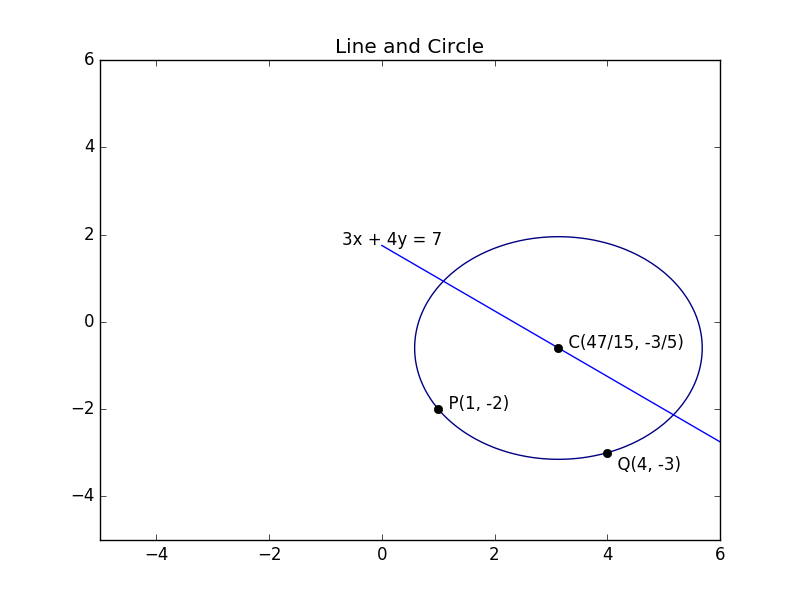
\includegraphics[width=11cm, height=7cm]{circle}
\end{document}
